\section{进阶扩展}
\begin{frame}[fragile]
\frametitle{数组公式运用(奇技淫巧,不建议常用)}
\begin{itemize}
		\item<+-> 一对多查找
		
		\begin{itemize}
			\item 万金油公式:\\
			|=INDEX(D:D,SMALL(IF($C$1:$C$8=$G$2,ROW($C$1:$C$8),100),ROW(A1)))&""|
		\end{itemize}
%	
		\item<+-> 去重复
		
		\begin{itemize}
			\item 删除重复项
			\item Power query
			\item 高级筛选
			\item 数据透视表
%			\item 数组公式
		\end{itemize}
\end{itemize}
\end{frame}


\begin{frame}[fragile]
	\frametitle{VBA入门及示例}
	\begin{itemize}
		\item 自定义函数
		\item 数组、字典组合
		\item SQL结合
	\end{itemize}
\end{frame}

\begin{frame}[fragile]
\frametitle{自定义函数(get\_price)}
	\begin{columns}
		\begin{column}{\textwidth}
		\begin{figure}		
%			\caption{获取单价get\_price函数}
			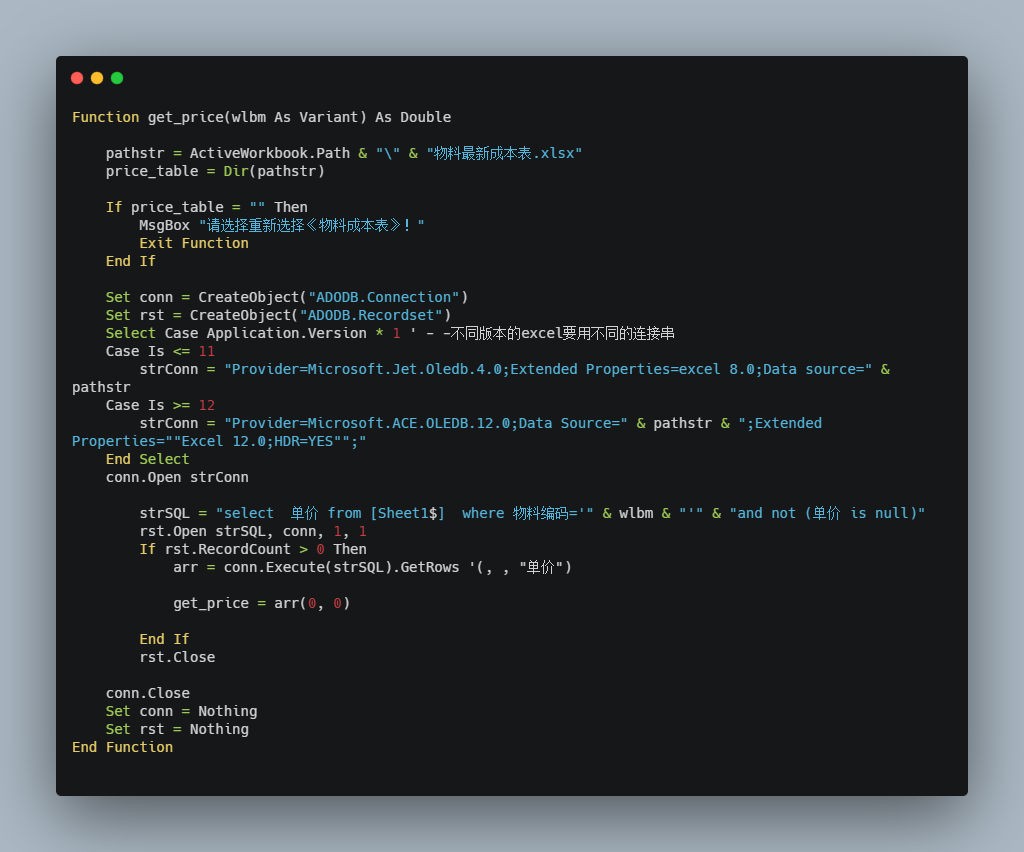
\includegraphics[height=\textheight]{figures/gprice.png}
		\end{figure}
		\end{column}
	\end{columns}
\end{frame}

\begin{frame}[fragile]
	\frametitle{自定义函数(getBomList)}
	\begin{columns}
		\begin{column}{\textwidth}
			\begin{figure}		
%				\caption{获取单价getBomList函数}
				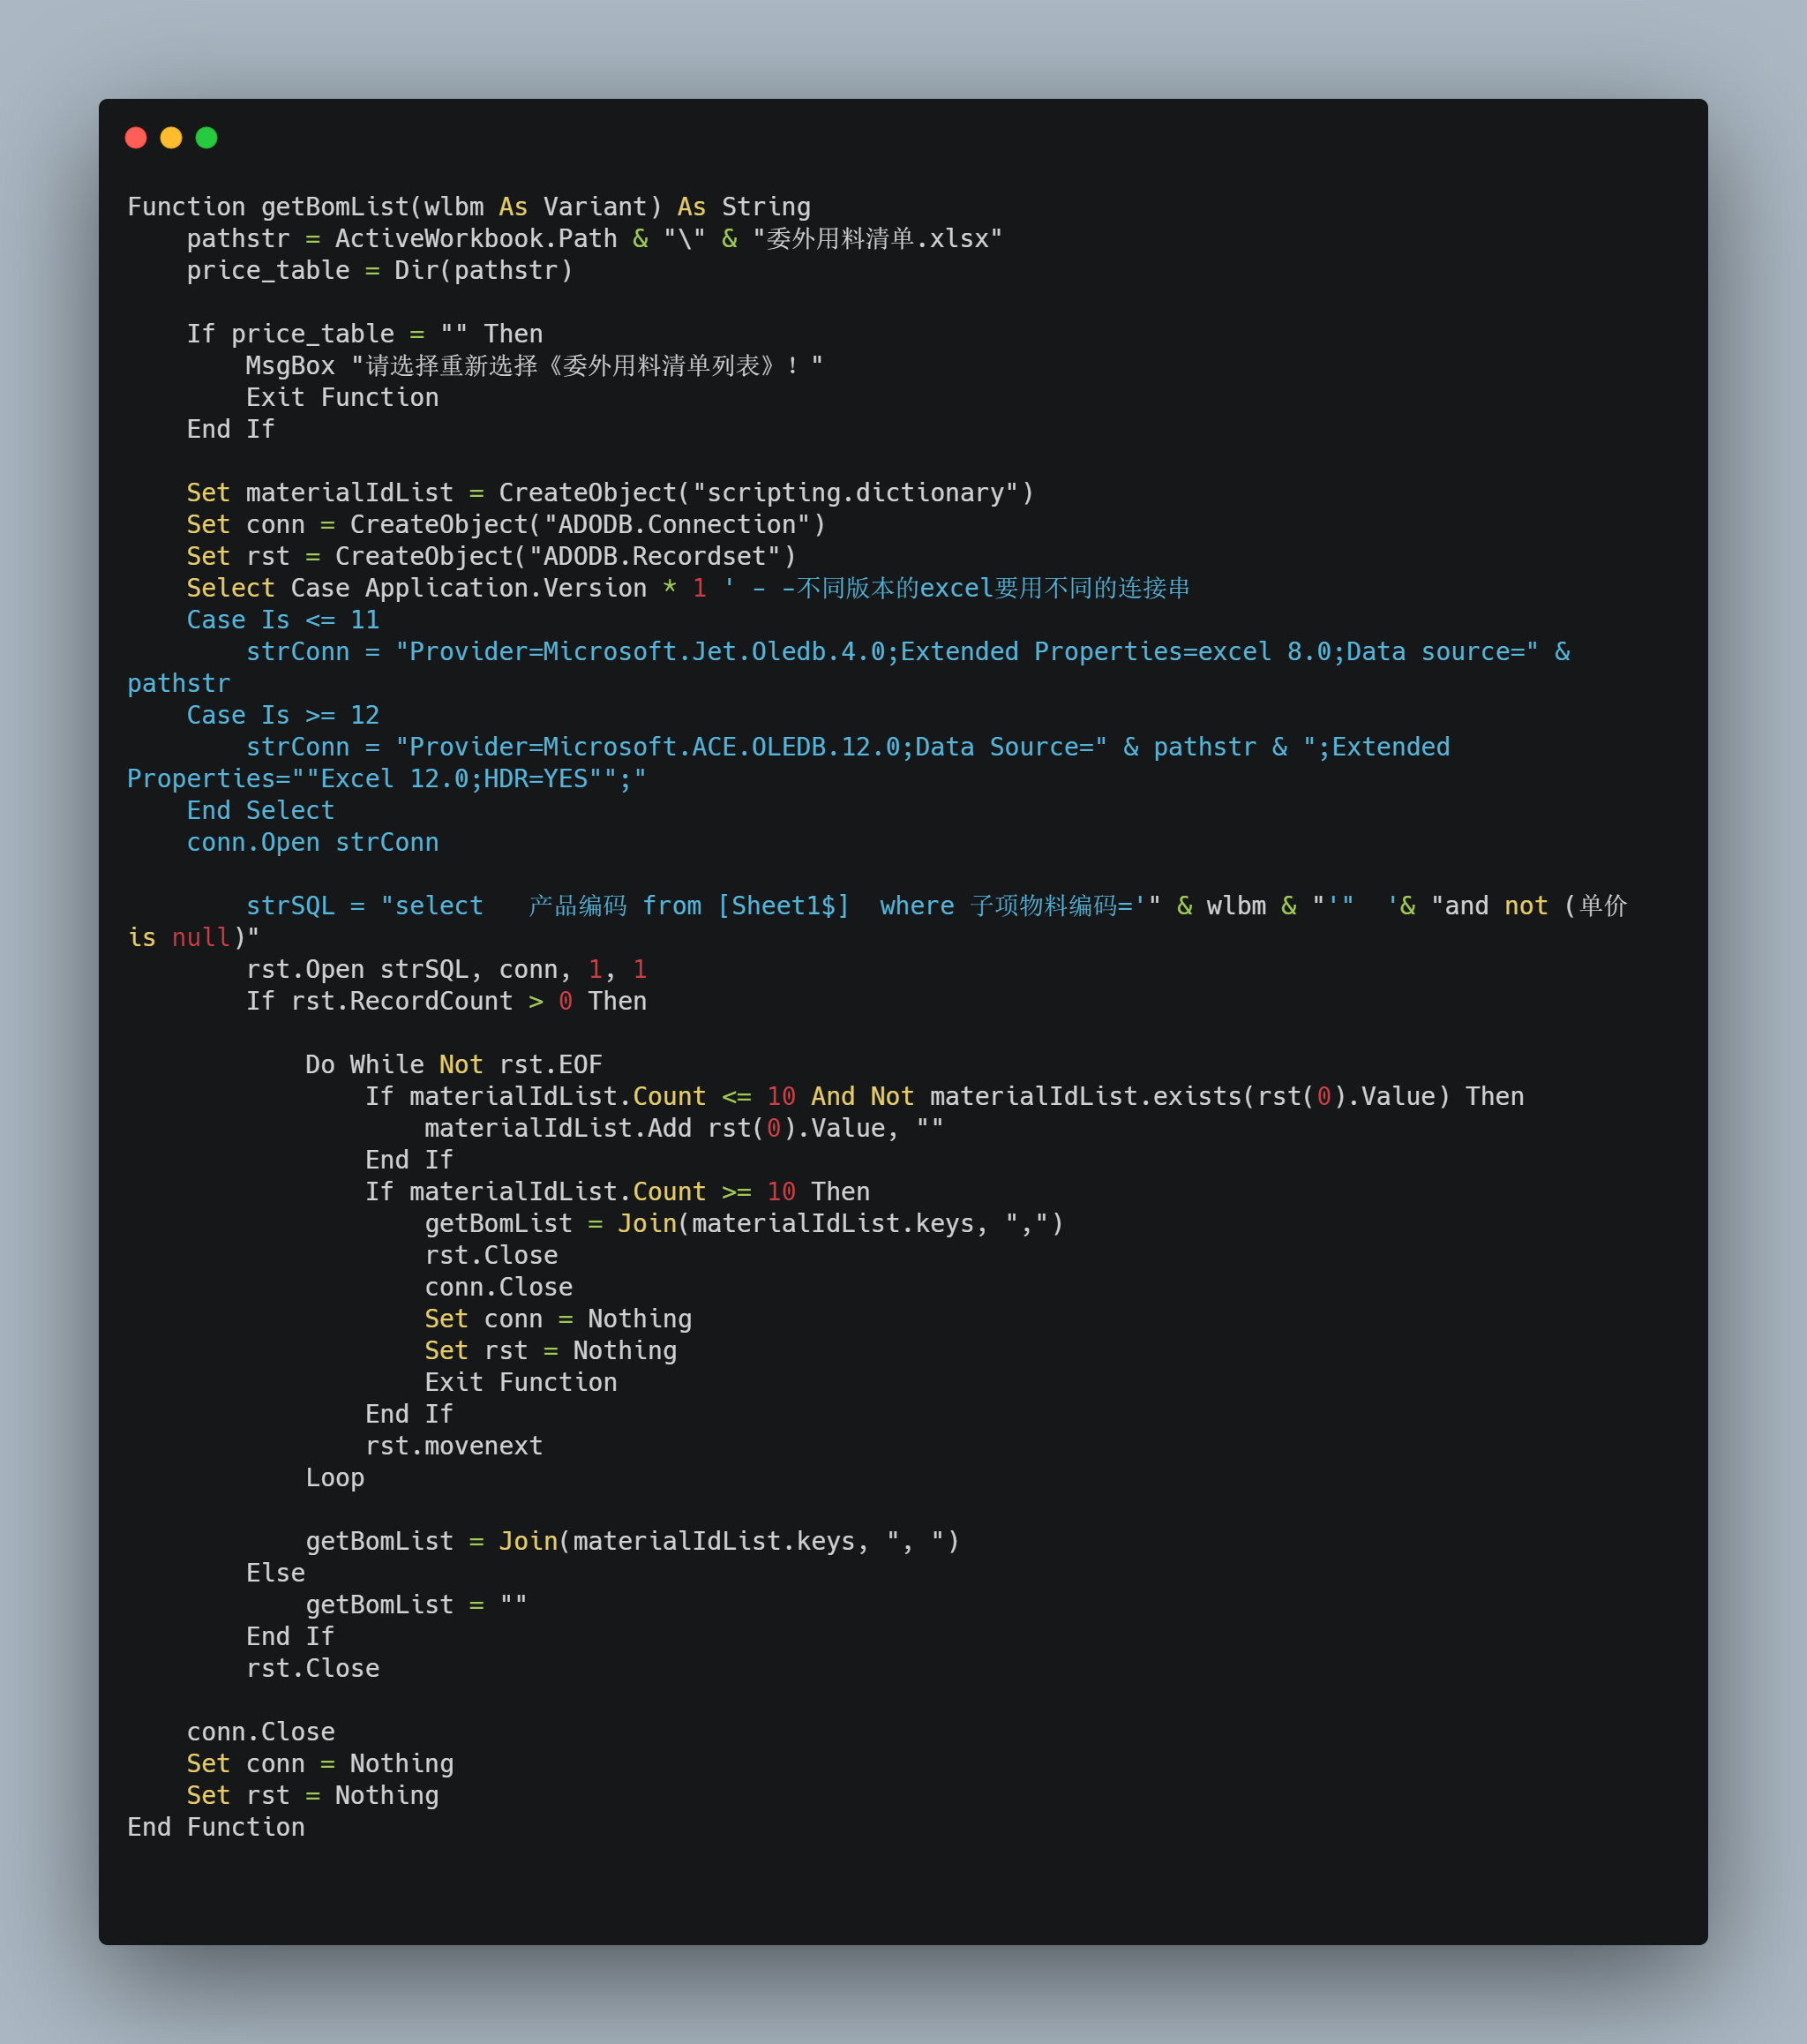
\includegraphics[height=\textheight]{figures/getBomList.png}
			\end{figure}
		\end{column}
	\end{columns}
\end{frame}

\begin{frame}[fragile]
	\frametitle{数组、字典组合应用}
	\begin{columns}
		\begin{column}{\textwidth}
			\begin{figure}		
				%				\caption{获取单价getBomList函数}
				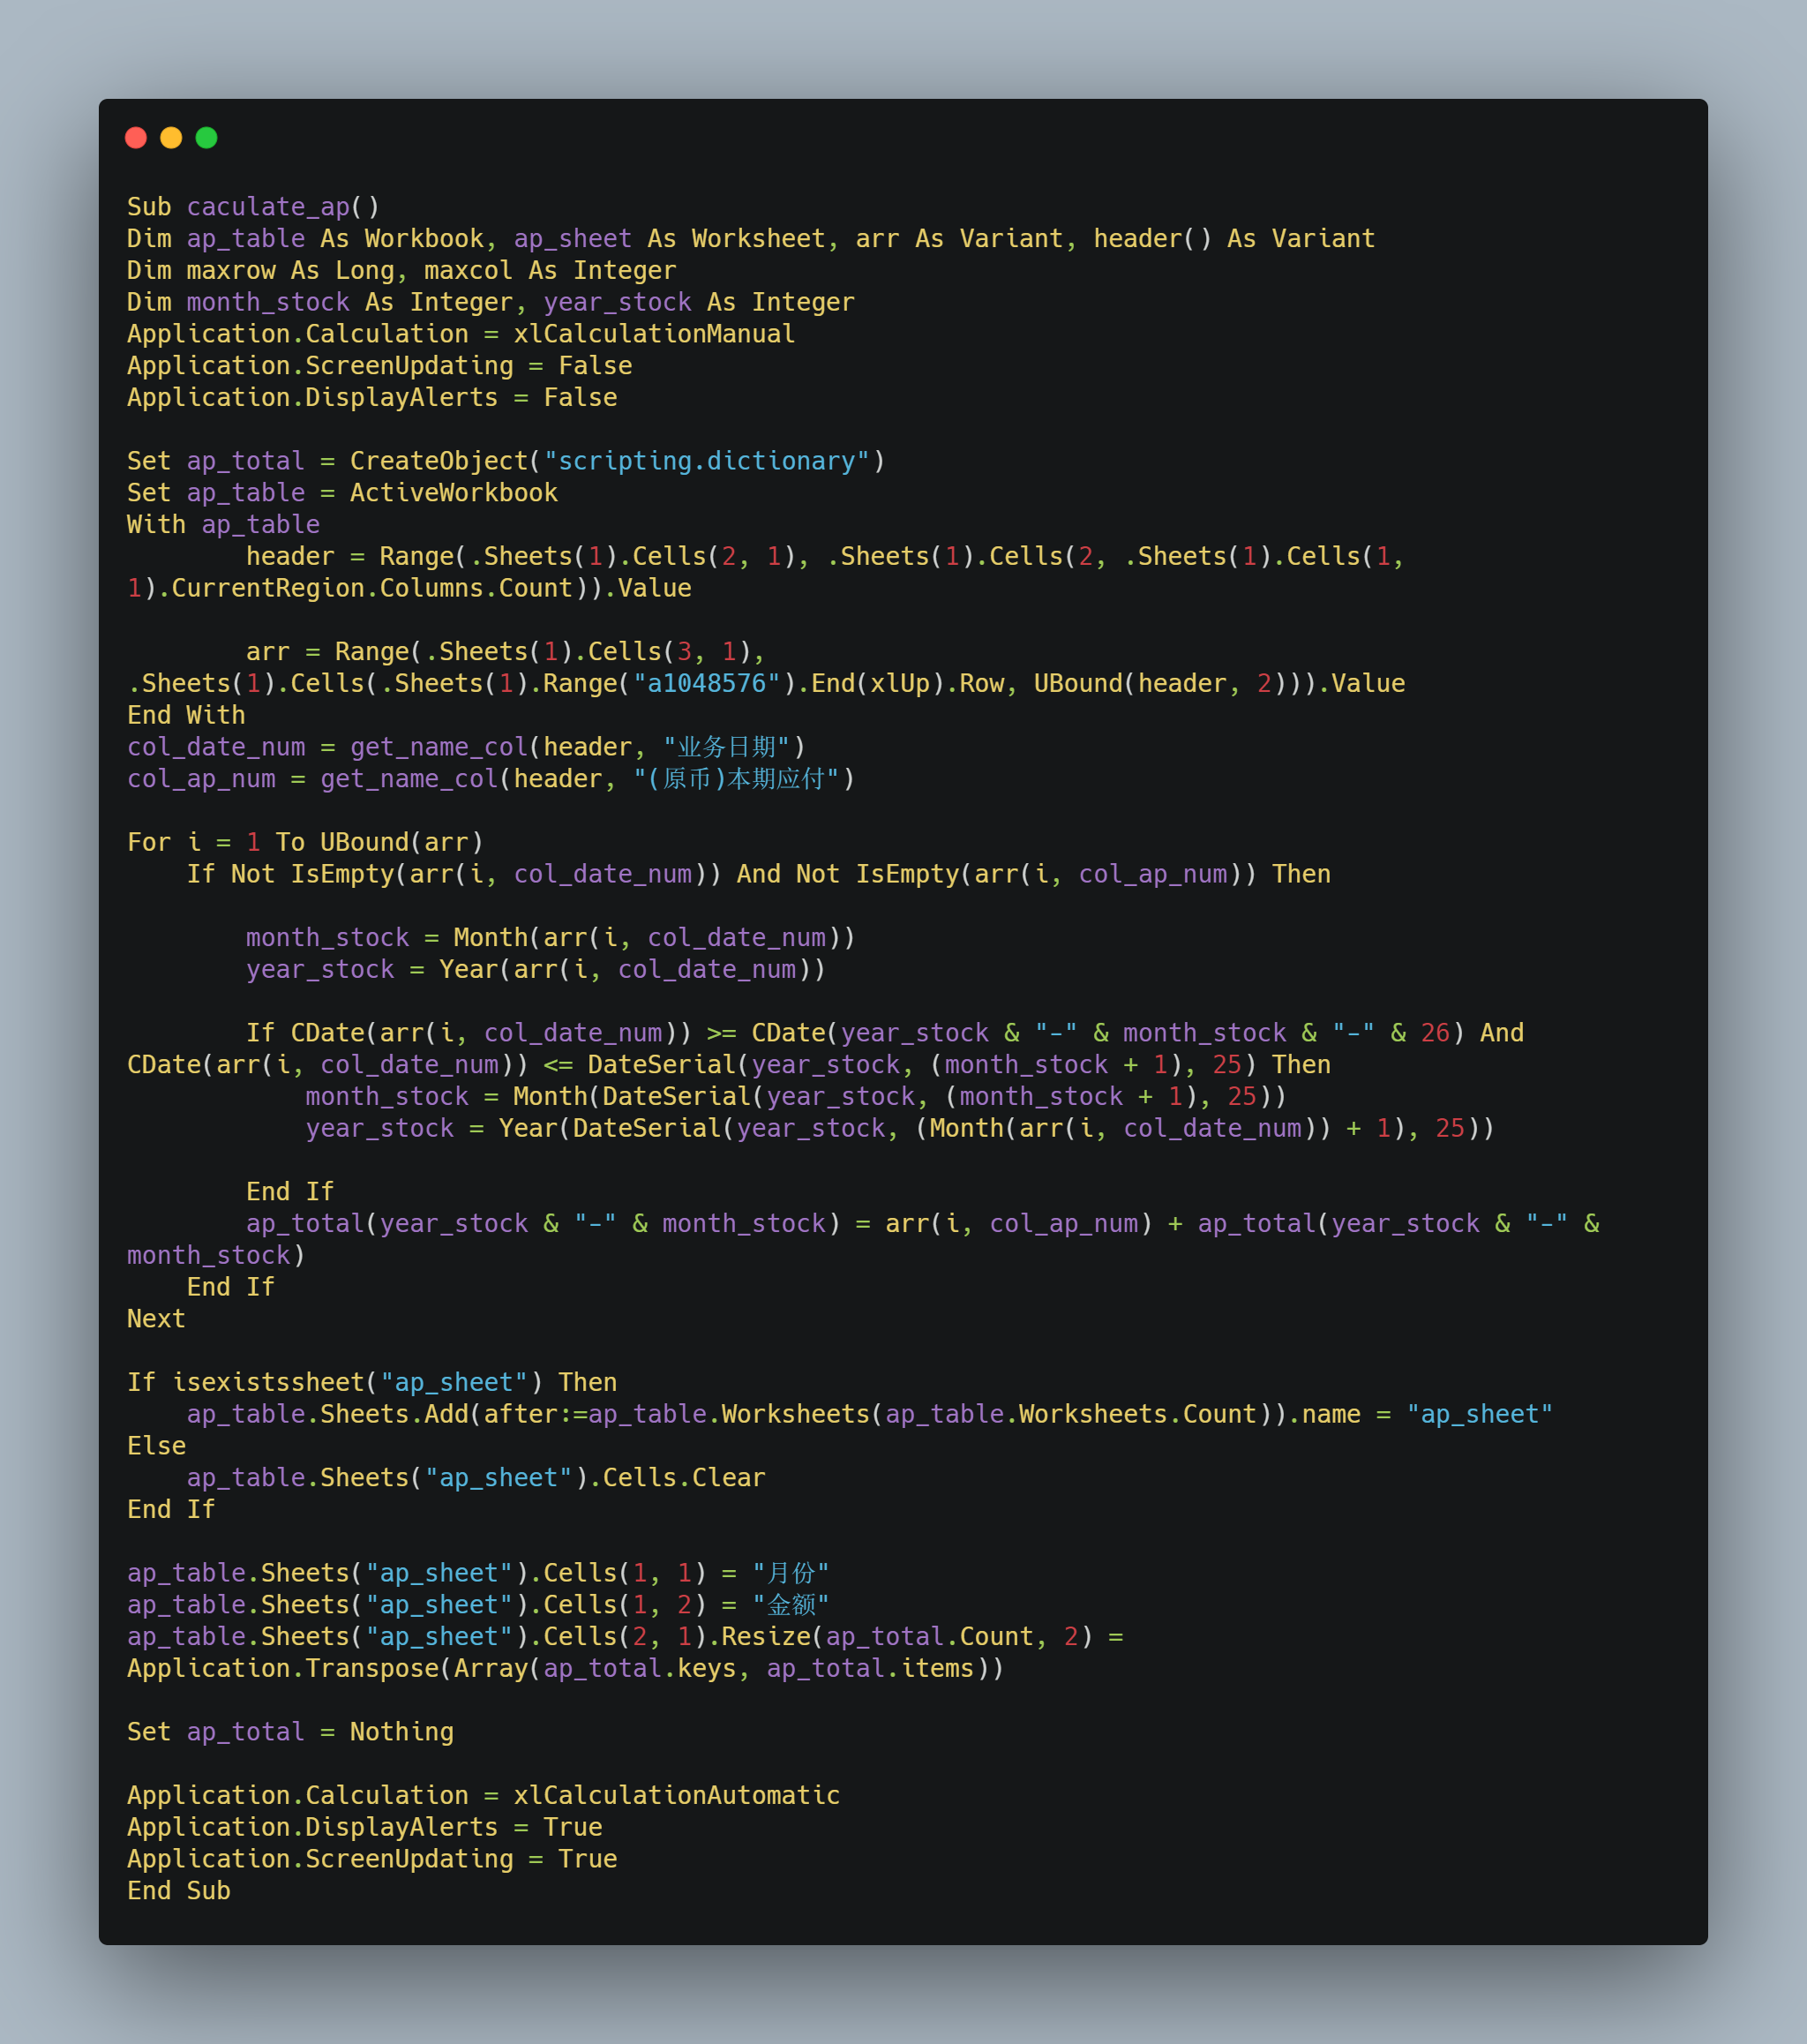
\includegraphics[height=\textheight]{figures/arr_dic.png}
			\end{figure}
		\end{column}
	\end{columns}
\end{frame}


\begin{frame}[fragile]
	\frametitle{Power Query运用示例}
	\begin{itemize}
		\item<+-> 常用操作
		\begin{itemize}
			\item 提升标题
			\item 更改数据类型
			\item 删除错误/空值
			\item 删除重复项
			\item 填充
			\item 合并列
			\item 拆分列
			\item 分组
			\item 提取
			\item 行列转置
			\item 行列操作
			\item 逆透视列
			\item 透视列
			\link{https://zhuanlan.zhihu.com/p/116461783}
		\end{itemize}
		\item<+-> 常用示例
		\begin{itemize}		
			\item 多表合并
			\item 多文件合并		
		\end{itemize}
	\end{itemize}
\end{frame}
%\begin{frame}[fragile]
%\frametitle{\TeX{} 宏编程}
%\begin{itemize}
%  \item<+-> \TeX{} 层面
%
%    \begin{itemize}
%      \item 守序善良——定义命令:|\def|、|\gdef|、|\let|
%      \item 绝对中立——展开控制:|\edef|、|\expandafter|、|\aftergroup|
%      \item 混乱邪恶——类别码:|\catcode|
%    \end{itemize}
%
%  \item<+-> \LaTeX{} 层面
%
%    \begin{itemize}
%      \item 定义新命令:|\newcommand|、|\renewcommand|、|\newenvironment|
%      \item 内部命令:|\makeatletter|、|\makeatother|
%    \end{itemize}
%
%  \item<+-> \LaTeX3——遥遥无期的未来
%
%    \begin{itemize}
%      \item 命令举例:|\cs_new:cpx|、|\seq_sort:Nn|、|\regex_match:nnTF|
%      \item 创建用户层命令:\pkg{xparse} 宏包
%      \item 面向对象编程:\pkg{xtemplate} 宏包
%      \item \pkg{fontspec}、\pkg{siunitx}、\pkg{ctex}、\pkg{fduthesis} 等均使用 \LaTeX3 实现
%    \end{itemize}
%
%  \item<+-> 外部语言调用
%
%    \begin{itemize}
%      \item |\write18|、|\directlua| 与 Python\TeX{}
%    \end{itemize}
%\end{itemize}
%\end{frame}
%
%\begin{frame}[fragile]
%\frametitle{深入字体}
%\begin{itemize}
%  \item<+-> NFSS 与字体的坐标
%
%    \begin{itemize}
%      \item 字体族、形状、系列、编码、字号
%      \item \TeX{} 仅需要 metric 信息:|.tfm|
%    \end{itemize}
%
%  \item<+-> 现代方案:OpenType
%
%    \begin{itemize}
%      \item 编码层面:支持 Unicode
%      \item 东亚文字:超大字符集、地区变体、竖排
%      \item 中东、南亚文字:Bi-di 文本、上下文连字、字符序调整
%    \end{itemize}
%
%  \item<+-> OpenType 中的数学支持(|MATH| 表)
%
%    \begin{itemize}
%      \item Unicode Math:字母、符号支持
%      \item 「数学常数」:整体度量信息——上下标位置、分数线粗细等
%      \item |MathVariants|:大小替换(积分号、根号、括号等)
%      \item |MathGlyphConstruction|:字符形装配(更大的根号、括号等)
%    \end{itemize}
%
%  \item<+-> 可变字体、\jatext{絵文字}%
%    \zhparen{emoji, \raisebox{-.2ex}{\includegraphics{example/emoji.pdf}}}……
%\end{itemize}
%\end{frame}
%
%\begin{frame}[fragile]
%\frametitle{编写宏包}
%\begin{itemize}
%  \item<+-> 文学编程
%
%    \begin{itemize}
%      \item 代码、注释与文档合为一体(|.dtx| 文件)
%      \item 使用 \pkg{doc} 与 \pkg{docstrip} 宏包
%    \end{itemize}
%
%  \item<+-> 发布
%
%    \begin{itemize}
%      \item 上传 CTAN 实际上并无门槛
%      \item 但仍有必要了解:
%
%        \begin{itemize}
%          \item \TeX{} 目录结构(TDS)
%          \item 测试系统:\pkg{l3build} 宏包
%          \item 版本控制、持续集成
%          \item 许可证选择:\LaTeX{} 内核使用 LPPL 1.3c
%            \link{https://www.latex-project.org/lppl/lppl-1-3c}
%        \end{itemize}
%    \end{itemize}
%
%  \item<+-> 参考
%
%    \begin{itemize}
%      \item \LaTeX{} 内核代码:\pkg{source2e.pdf}、\pkg{classes.pdf}、\pkg{source3.pdf}
%      \item 书籍:\emph{The \TeX book}、\emph{\TeX{} by Topic}、\emph{The \LaTeX{} Companion} 等
%    \end{itemize}
%\end{itemize}
%\end{frame}
%
%\begin{frame}[fragile]
%\frametitle{宏包推荐}
%\footnotesize
%\setbeamertemplate{itemize/enumerate subbody begin}{\scriptsize}
%\setlength{\leftmarginii}{1.5em}
%\begin{multicols}{3}
%  \begin{itemize}
%    \item 必备
%
%      \begin{itemize}
%        \item \pkg{amsmath}
%        \item \pkg{graphicx}
%        \item \pkg{hyperref}
%      \end{itemize}
%
%    \item 样式
%
%      \begin{itemize}
%        \item \pkg{caption}
%        \item \pkg{enumitem}
%        \item \pkg{fancyhdr}
%        \item \pkg{footmisc}
%        \item \pkg{geometry}
%        \item \pkg{ntheorem}
%        \item \pkg{titlesec}
%      \end{itemize}
%
%    \item 数学
%
%      \begin{itemize}
%        \item \pkg{bm}
%        \item \pkg{mathtools}
%        \item \pkg{physics}
%        \item \pkg{unicode-math}
%      \end{itemize}
%
%    \item 表格
%
%      \begin{itemize}
%        \item \pkg{array}
%        \item \pkg{booktabs}
%        \item \pkg{longtable}
%        \item \pkg{tabularx}
%      \end{itemize}
%
%    \item 插图、绘图
%
%      \begin{itemize}
%        \item \pkg{float}
%        \item \pkg{pdfpages}
%        \item \pkg{standalone}
%        \item \pkg{subfig}
%        \item \pkg{pgf}/\pkg{tikz}
%        \item \pkg{pgfplots}
%      \end{itemize}
%
%    \item 字体
%
%      \begin{itemize}
%        \item \pkg{newtx}
%        \item \pkg{newpx}
%        \item \pkg{pifont}
%        \item \pkg{fontspec}
%      \end{itemize}
%
%    \item 多语言
%
%      \begin{itemize}
%        \item \pkg{babel}
%        \item \pkg{polyglossia}
%        \item \pkg{ctex}
%        \item \pkg{xeCJK}
%        \item \pkg{luatexja}
%      \end{itemize}
%
%    \item 杂项功能
%
%      \begin{itemize}
%        \item \pkg{algorithm2e}
%        \item \pkg{beamer}
%        \item \pkg{biblatex}
%        \item \pkg{fancyhdr}
%        \item \pkg{listings}
%        \item \pkg{mhchem}
%        \item \pkg{microtype}
%        \item \pkg{minted}
%        \item \pkg{natbib}
%        \item \pkg{siunitx}
%        \item \pkg{xcolor}
%      \end{itemize}
%  \end{itemize}
%\end{multicols}
%\vspace*{-0.5cm}
%\end{frame}
%
%\begin{frame}[standout]
%  \huge \textbf{请务必先读文档!} \\[1ex] \pause
%  \footnotesize 命令行执行 \texttt{texdoc \textit{package}}
%\end{frame}
%
%\begin{frame}[fragile]
%\frametitle{Markdown}
%\begin{columns}
%\lstset{%
%  moredelim    = [s][emphstyle]{*}{*},
%  moredelim    = [s][keywordstyle]{**}{**},
%  moredelim    = [s][emphstyle2]{\`}{\`},
%  moredelim    = [s][emphstyle2]{\`\`\`}{\`\`\`},
%  moredelim    = [l][keywordstyle2]{\#},
%  moredelim    = [is][keywordstyle2]{+}{+},
%  moredelim    = *[is][\itshape]{!}{!},
%  moredelim    = [is][keywordstyle]{(+}{+)},
%  moredelim    = [is][emphstyle2]{(-}{-)},
%  basicstyle   = \scriptsize\ttfamily,
%  keywordstyle = [1]\bfseries\color{keyword},
%  keywordstyle = [2]\bfseries\color{texcs},
%  emphstyle    = [1]\itshape\color{emph1},
%  emphstyle    = [2]\color{inline}}
%\begin{column}{0.5\textwidth}
%  \begin{lstlisting}[gobble=2]
%  # Markdown syntax
%
%  This is **bold text**.
%  This text is *italicized*.
%  Use `git status` to list all
%  new or modified files.
%
%  Block code:
%
%  ```
%  git status
%  git add
%  git commit
%  ```
%
%  Quotation:
%
%  +>+ !Markdown uses email-style `>`!
%  +>+ !characters for blockquoting.!
%  \end{lstlisting}
%\end{column}
%\begin{column}{0.5\textwidth}
%  \begin{lstlisting}[gobble=2]
%  ## List
%
%  ### Bullet list
%
%    +*+ apples
%    +*+ oranges
%    +*+ pears
%
%  ### Numbered list
%
%    +1.+ wash
%    +2.+ rinse
%    +3.+ repeat
%
%  +---+
%
%  Link: from [(+Wikipedia+)]
%  ((-https://en.wikipedia.org/wiki/-)
%  (-Markdown-))
%
%  \end{lstlisting}
%\end{column}
%\end{columns}
%\vspace{-0.6cm}
%\end{frame}
%
%\begin{frame}[fragile]
%\frametitle{Git}
%\begin{itemize}
%  \item<+-> 版本管理的必要性
%
%    \begin{itemize}
%      \item 远离「初稿,第二稿,第三稿……终稿,终稿(打死也不改了)」
%      \item 有底气做大范围修改、重构
%      \item 方便与他人协同合作
%    \end{itemize}
%
%  \item<+-> 基本用法
%
%    \begin{itemize}
%      \item 把大象放进冰箱:|git init|、|git add|、|git commit|
%      \item 时空穿梭:|git reset|、|git revert|
%      \item 平行宇宙:|git branch|、|git checkout|、|git rebase|
%      \item 推荐用 VS Code 等进行可视化操作
%      \item 参考链接:\link{https://git-scm.com/book/en/v2}
%        \link{https://www.liaoxuefeng.com/wiki/0013739516305929606dd18361248578c67b8067c8c017b000}
%    \end{itemize}
%
%  \item<+-> GitHub \href{https://github.com}{\faGithub}
%
%    \begin{itemize}
%      \item 远程 Git 仓库
%      \item Clone \& fork
%      \item Issues \& pull requests
%      \item<+-> \alert{提醒:绑定 \texttt{.edu} 邮箱可以免费无限量使用私有仓库}
%    \end{itemize}
%\end{itemize}
%\end{frame}
%
%\begin{frame}[fragile]
%\frametitle{参考文献}
%\begin{multicols}{2}
%\tiny
%\newcommand\BOOK[1]{\textbf{#1}}
%\newcommand\TAG[1]{\CASE{[#1]}}
%\begin{thebibliography}{99}
%  \bibitem{}
%    \textsc{Knuth D E}.
%    \newblock \BOOK{The \TeX book: Computers \& Typesetting, volume C} \TAG{M}. 1984.
%    \newblock Boston: Addison--Wesley Publishing Company
%  \bibitem{}
%    刘海洋.
%    \newblock \BOOK{\LaTeX{} 入门} \TAG{M}. 2013.
%    \newblock 北京:电子工业出版社
%  \bibitem{}
%    \jatext{高冈昌生}.\\
%    翻译:刘庆,监修:陈嵘.
%    \newblock \BOOK{西文排版:排版的基础和规范} \TAG{M}. 2016.
%    \newblock 北京:中信出版集团
%  \bibitem{}
%    \jatext{小林章}.\\
%    翻译:刘庆,监修:陈嵘.
%    \newblock \BOOK{西文字体:字体的背景知识和使用方法} \TAG{M}. 2014.
%    \newblock 北京:中信出版集团
%  \bibitem{}
%    \textsc{Oetiker T}, \textsc{Partl H}, \textsc{Hyna I} and \textsc{Schlegl E}.\\
%    翻译:\CTeX{} 开发小组.
%    \newblock \BOOK{一份(不太)简短的 \LaTeXe{} 介绍:或 110 分钟了解 \LaTeXe{}} \TAG{EB/OL}. 2019.
%    \newblock \url{https://ctan.org/pkg/lshort-zh-cn}
%  \bibitem{}
%    汪彧之,陈晟祺.
%    \newblock \BOOK{如何使用 \LaTeX{} 排版论文} \TAG{EB/OL}. 2019.
%    \newblock PDF:
%      \href{https://github.com/tuna/thulib-latex-talk/raw/master/latex-talk.pdf}{\faDownload}
%  \bibitem{}
%    刘海洋.
%    \newblock \BOOK{\LaTeX{} 入门} \TAG{EB/OL}. 2013.
%    \newblock PDF:
%      \href{https://bbs.pku.edu.cn/attach/e7/f2/e7f2bb698b9c3672/tex_intro_talk.pdf}{\faDownload}
%  \bibitem{}
%    林莲枝.
%    \newblock \BOOK{漫谈 \LaTeX{} 排版常见概念误区:别把 \LaTeX{} 当 Word 用!}\TAG{EB/OL}. 2018.
%    \newblock PDF:
%      \href{http://static.latexstudio.net/wp-content/uploads/2018/03/LianTze-presentation-0320-forReading.pdf}{\faDownload}
%  \bibitem{}
%    Wikibooks.
%    \newblock \BOOK{\LaTeX{}---Wikibooks, The Free Textbook Project} \TAG{EB/OL}.
%    \newblock \url{https://en.wikibooks.org/wiki/LaTeX}
%  \bibitem{}
%    Overleaf.
%    \newblock \BOOK{Overleaf Documentation} \TAG{EB/OL}.
%    \newblock \url{https://www.overleaf.com/learn}
%  \bibitem{}
%    刘庆.
%    \newblock \BOOK{孔雀计划:中文字体排印的思路} \TAG{EB/OL}.
%    \newblock \url{https://thetype.com/kongque}
%\end{thebibliography}
%\end{multicols}
%\end{frame}
